\section{Physical Simulation}

\subsection{Dynamics Equations}

We model the robot as an articulated rigid body system in our simulator. We represent the states of the system $(\mathbf{x}, \dot{\mathbf{x}})$ in generalized coordinates, where $\mathbf{x}$ includes the global position $\mathbf{p}$, the orientation $\mathbf{r}$ of the root body (robot's torso), and the joint angles $\mathbf{q}$. The dynamics equations is as follows:

\begin{equation}
\label{eq:robotdynamics}
\mathbf{M}(\mathbf{x})\mathbf{\ddot{x}}+\mathbf{C}(\mathbf{x},\mathbf{\dot{x}})=\boldsymbol{\tau}(\mathbf{q}, \dot{\mathbf{q}}, \bar{\mathbf{q}})+\mathbf{J}^T\mathbf{f}
\end{equation}
where $\mathbf{M}(\mathbf{x})$ is the mass matrix and $\mathbf{C}(\mathbf{x},\mathbf{\dot{x}})$ is the Coriolis and Centrifugal force. $\boldsymbol{\tau}(\mathbf{q}, \dot{\mathbf{q}}, \bar{\mathbf{q}})$ are joint torques exerted by the actuators, which depends on the current joint angles $\mathbf{q}$, velocities $\dot{\mathbf{q}}$ and desired angles $\bar{\mathbf{q}}$. The relation between these quantities is determined by the actuator model, which is presented in the next section. $\mathbf{J}$ is the Jacobian matrix and $\mathbf{f}$ is the external contact force, which is computed based on linear complementarity conditions \cite{Tan:2012b}. In our implementation, we use DART to solve the contact force and numerically integrate the system state $(\mathbf{x}, \dot{\mathbf{x}})$ over time.
\ignorethis{
  /karen{Make actuator modeling sound important. Argue why we had to build an accurate model for actuator instead of improving other sources of simulation errors.}
  }

\subsection{Actuator Model}
\label{sec:motorDynamics}
A faithful robot simulation relies heavily on an accurate actuator model. A common practice is to set the same PID gains in the simulation as those in the servo. However, Dynamixel AX-18 servos, used on our robot (ROBOTIS BIOLOID GP), do not support PID control. Although the servo can track an input desired angle $\bar{q}$, the relation between the joint error $\bar{q}-q$ and the output torque $\tau$ is unclear. We derive an actuator model based on the ideal DC motor assumption and the specification of the servo:

\begin{equation}
  \tau = -k_p(q-\bar{q}) - k_d\dot{q} - k_c\sgn(\dot{q})\\
    \label{eqn:torqueErrorRelationSimple}
\end{equation}
We call $k_p$, $k_d$ and $k_c$ the \emph{actuator gains}. Note that these are not PID gains. These gains are determined by the design of the servo, which are unknown to us. The detailed derivation of the actuator model (eq. (\ref{eqn:torqueErrorRelationSimple})) can be found in Appendix.

We design a robot experiment to estimate the actuator gains $k_p$, $k_d$ and $k_c$. The purpose of this simple experiment is not to accurately identify these values. Instead, the gains that we estimate here will serve as an initial guess, and will be further optimized in simulation calibration. In the experiment, we clamp the entire robot on a table except for the left foot. We then send a periodic control signal $\bar{q}(t)$ to the servo at the left ankle (blue curve in Figure \ref{fig:actuatorId}). The desired joint angle stays at the maximum value for 0.67 second, then changes to the minimum value and stays for another 0.67 second and repeats. We record the trajectory of the actual joint angle $q(t)$ throughout the experiment (green curve in Figure \ref{fig:actuatorId}). 

\begin{figure}[!t]
  \centering
  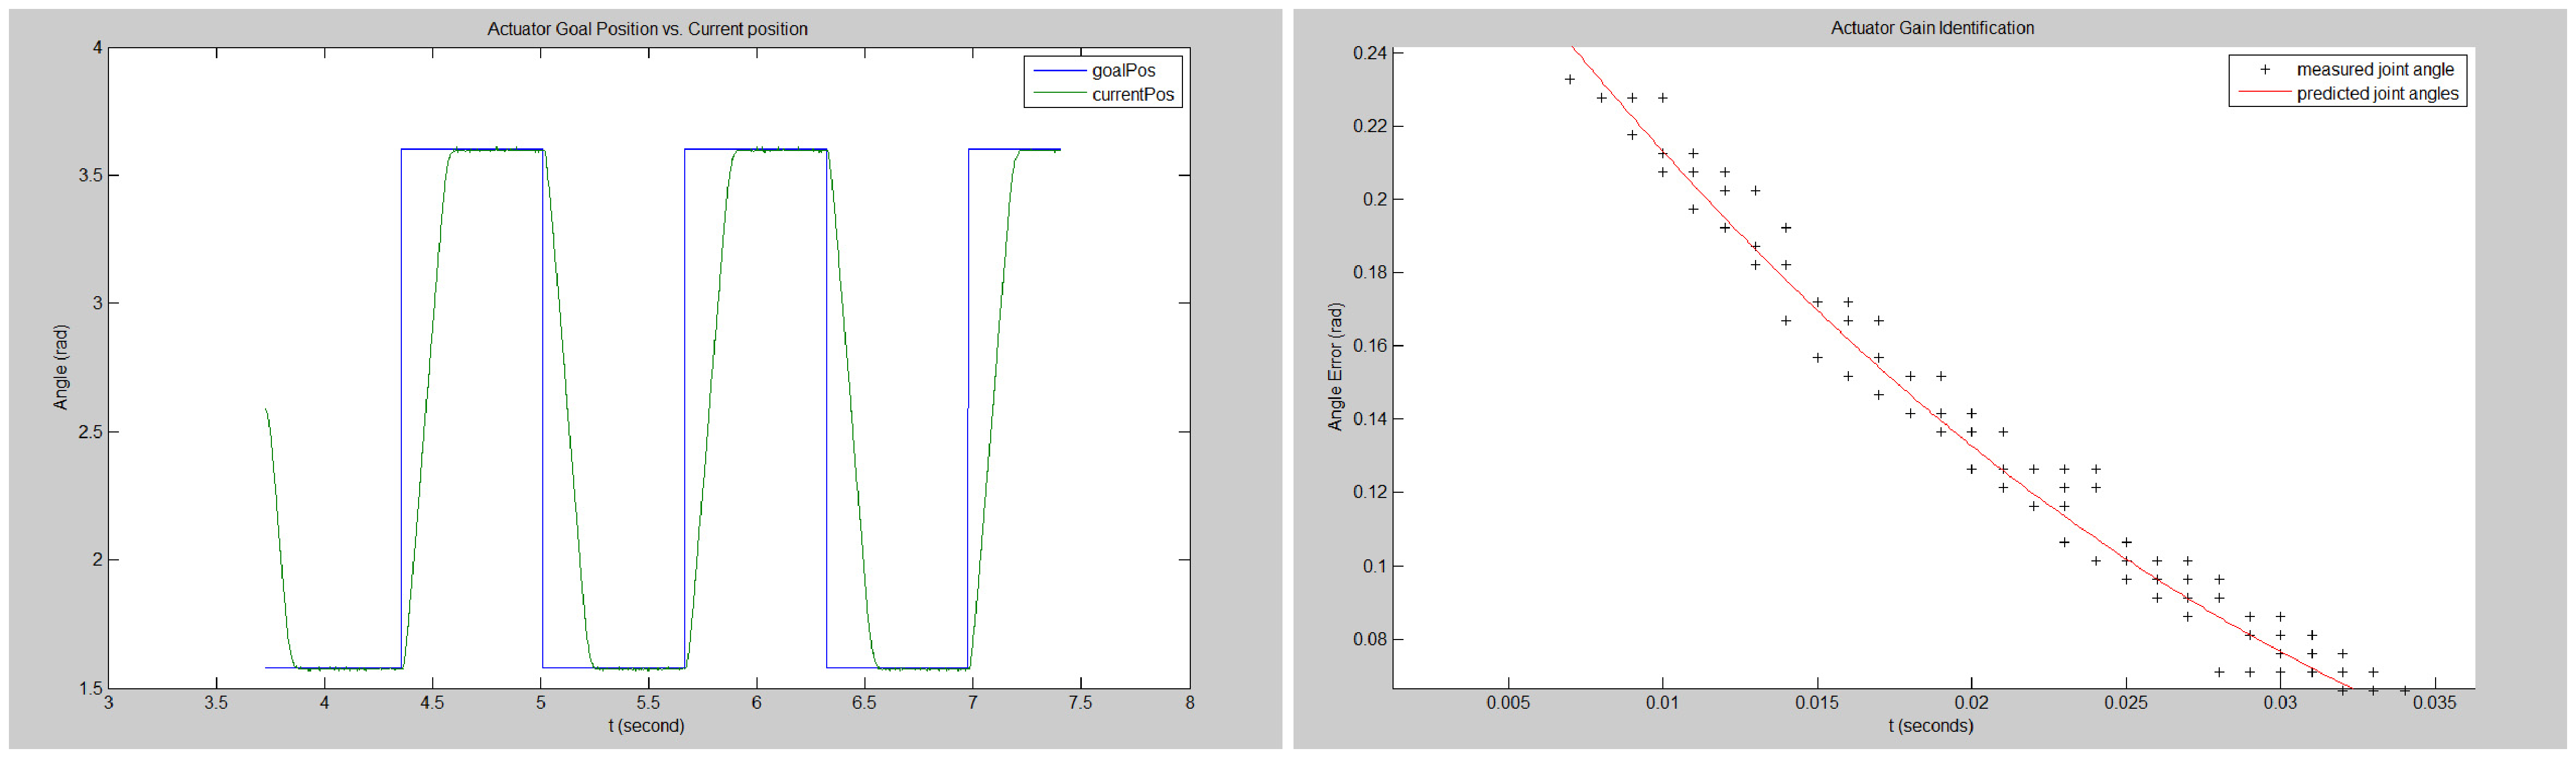
\includegraphics[width=0.3\textwidth]{figures/actuatorId}
  \caption{The trajectories of the desired and the measured joint angle for acutator identification.}
  \vspace{-0.1in}
  \label{fig:actuatorId}
\end{figure}

Given $q(t)$ and $\bar{q}(t)$, we apply regression to estimate the actuator gains:

\begin{displaymath}
\min_{k_p, k_d, k_c}\int||I\ddot{q}(t)+k_p(q(t)-\bar{q}(t)) + k_d\dot{q}(t) + k_c\sgn(\dot{q}(t))||^2\mathrm{d}t
\end{displaymath}
where $I$ is the moment of inertia of the foot with respect to the rotating axis. The above equation is derived by plugging into $\tau = I\ddot{q}+\dot{I}\dot{q}$ and the fact that $\dot{I}\dot{q}=0$ because the foot is a rigid body that rotates along a fixed axis. Our experiments and computation show that the actuator gains are $k_p=9.272(N\cdot m/rad)$, $k_d=0.3069(N\cdot m\cdot s/rad)$, and $k_c=0.03(N\cdot m)$. 


